\chapter[ಅಧ್ಯಾಯ 5]{}\label{chap5}

\begin{center}
\rule{5cm}{1pt}\\[5pt]
{\Large\bfseries ಸಮಸ್ಯೆಗಳು}\\[3pt]
\rule{5cm}{1pt}
\end{center}

\begin{enumerate}
\renewcommand{\labelenumi}{\bf\theenumi.}
\itemsep=5pt

\item ಏಳು 4 ಬಳಸಿ 100 ಬರಿಸಿ (ಯಾವುದೇ ಗಣಿತ ಚಿಹ್ನೆ ಬಳಸಬಹುದು)

\item 5 ಸಂಖ್ಯೆಗಳಿವೆ 16, 17, 23, 24, 29. ಯಾವ ಸಂಖ್ಯೆ ಎಷ್ಟು ಬಾರಿ ಬೇಕಾದರೂ ಬಳಸಿ 100 ಮೊತ್ತ ಬರಿಸಿ.  

\item ಆರು 3 ಬಳಸಿ 8 ಬರಿಸಿ

\item ಐದು ಸಲ 4 ಬಳಸಿ 55 ಬರಿಸಿ 

\item ನನಗೆ ಕಾಣದಂತೆ 2 ಅಂಕಿ ಸಂಖ್ಯೆ ಬರೆಯಿರಿ. ವರ್ಗ ಮಾಡಿ ಮೊದಲ ಸಂಖ್ಯೆಗೆ 6 ಕೂಡಿಸಿ, ವರ್ಗಮಾಡಿ. ಎರಡು ವರ್ಗಗಳ ವ್ಯತ್ಯಾಸ ಹೇಳಿ. ನಿಮ್ಮ ಸಂಖ್ಯೆ ಹೇಳುತ್ತೇನೆ

\item ನನಗೆ ಕಾಣದಂತೆ ಮೂರಂಕಿ ಸಂಖ್ಯೆ ಬರೆಯಿರಿ. ನೂರರ ಸ್ಥಾನದ ಅಂಕಿಯನ್ನು 2 ರಿಂದ ಗುಣಿಸಿ 1 ನ್ನು ಕೂಡಿ. ಉತ್ತರವನ್ನು 5 ರಿಂದ ಗುಣಿಸಿ 10 ರ ಸ್ಥಾನದ ಅಂಕಿ ಕೂಡಿಸಿ. 10 ರಿಂದ ಗುಣಿಸಿ. ಉತ್ತರಕ್ಕೆ ಬಿಡಿ ಸ್ಥಾನದ ಅಂಕಿ ಕೂಡಿಸಿ. ಉತ್ತರ ಹೇಳಿ. ನಿಮ್ಮ ಮೂರಂಕಿ ಸಂಖ್ಯೆ ಹೇಳುತ್ತೇನೆ.

\item ಒಂದು ಗೆರೆ ಸ್ಥಾನ ಪಲ್ಲಟ ಮಾಡಿ ಸಮೀಕರಣ ಸರಿದೂಗಿಸಿ $\neq$ ಬಳಸುವಂತಿಲ್ಲ.

\begin{tabular}{l@{\,}ll@{\,}l}
(a)& III $-$ I = III &(b) & VI $+$ V = IX\\
(c)& VI $-$ II = II &(d) & IV = III $-$ I\\
(e)& XI $+$ I = X~~(ಎರಡು ಉತ್ತರಗಳಿವೆ) & &
\end{tabular}

\eject

\item 16 ಬೆಂಕಿಕಡ್ಡಿ ಜೋಡಣೆ ಹೀಗಿದೆ.
\begin{figure}[H]
\centering
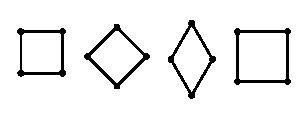
\includegraphics[scale=.9]{images/chap5/q8.eps}
\end{figure} 

4 ಕಡ್ಡಿ ತೆಗೆದು ಹಾಕಿ, 1 ನ್ನು ಸ್ಥಳಾಂತರಿಸಿ ``ಪ್ರೇಮ ಪದ" (ಇಂಗ್ಲಿಷಿನ) ಬರಿಸಿ.  

\item 8 ಬೆಂಕಿಕಡ್ಡಿಗಳಿಂದ ಈ ಆಕೃತಿ ರಚಿಸಿದೆ. 2 ಕಡ್ಡಿ ತೆಗೆದು 3 ಚೌಕ 2 ಆಯತ ಬರಿಸಿ.

\begin{figure}[H]
\centering
\includegraphics{images/chap5/q9.eps}
\end{figure}

\item  3 ಬೆಂಕಿಕಡ್ಡಿಗಳಿಂದ ಒಂದು ಸಮಬಾಹು ತ್ರಿಭುಜ ರಚಿಸಬಹುದು. 12 ಬೆಂಕಿಕಡ್ಡಿ  ಬಳಸಿ, ಸಮಾನ ಅಳತೆಯ 6 ತ್ರಿಭುಜ ರಚಿಸಿ. ನಂತರ 4 ಕಡ್ಡಿ ಸ್ಥಳಾಂತರಿಸಿ, 3 ಸಮಬಾಹು ತ್ರಿಭುಜ (ಒಂದೇ ಅಳತೆಯವಲ್ಲ) ಬರಿಸಿ.

\item 
\begin{itemize}
\item[(a)] 10 ಬೆಂಕಿಕಡ್ಡಿಗಳಿಂದ 3 ಲಗತ್ತಾಗಿರುವ ಚೌಕ ಬರಿಸಿ.
\item[(b)] ಅದರಲ್ಲಿ 1 ಕಡ್ಡಿ ತೆಗೆದು ಹಾಕಿ. ಒಂದು ಚೌಕ ಹಾಗೇ ಉಳಿಸಿ ಅದಕ್ಕೆ ಲಗತ್ತಾದ 2 ವಜ್ರಾಕೃತಿ ಬರುವಂತೆ ಕಡ್ಡಿಗಳನ್ನು ಹೊಂದಿಸಿ.  
\end{itemize}

\item 26 ಬೆಂಕಿಕಡ್ಡಿಗಳಿಂದಾದ ಜಾಲರಿ ಇದೆ. 

14 ಕಡ್ಡಿ ಸ್ಥಳಾಂತರಿಸಿ 3 ಚೌಕ ಬರಿಸಿ. 

\begin{figure}[H]
\centering
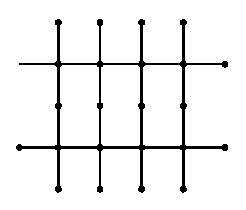
\includegraphics[scale=1.1]{images/chap5/q12.eps}
\end{figure}

\item ಈ ಗುಣಾಕಾರ ಗಮನಿಸಿ ಮುಂದಿನ 5 ಹಂತ ಬರೆಯಿರಿ. 

\begin{tabular}{l@{\;}l}
$9999\times 2$ & = $1998$\\
$9999\times 3$ & = $29997$\\
$9999\times 4$ & = $39996$
\end{tabular} 

\item ಇದನ್ನು ಗಮನಿಸಿ 
\begin{align*}
121 & = \dfrac{22\times 22}{1 + 2 + 1}\\
12321 & = \dfrac{333 \times 333}{1 + 2 + 3 + 2 + 1}
\end{align*}  

ಮುಂದಿನ ಹಂತ ಬರೆಯಿರಿ. 

\item ಇದನ್ನು ಗಮನಿಸಿ 

\begin{tabular}{c@{\;}c@{\;}c}
$3\times 5$ & = & $15$\\
$33\times 35$ & = & $1155$\\
$333 \times 335$ & = & $111555$
\end{tabular}

ಮುಂದಿನ 4 ಹಂತ ಬರೆಯಿರಿ. 

\item ಇದನ್ನು ಗಮನಿಸಿ.

\begin{tabular}[[t]{r@{\;}c@{\;}c}
$201^{2}$ & = & $40401$\\
$2001^{2}$ & = & $4004001$\\
$20001^{2}$ & = & $400040001$
\end{tabular}

ಮುಂದಿನ 3 ಹಂತ ಬರೆಯಿರಿ. 

\item $2^{5} \cdot 9^{2} = 2592$ ಇದರ ವಿಶಿಷ್ಟತೆ ಗಮನಿಸಿ 

\item 12 ತೆಂಗಿನ ಸಸಿಗಳಿವೆ ಸಾಲಿಗೆ 4 ಸಸಿ ಬರುವಂತೆ 6 ಸಾಲುಗಳಲ್ಲಿ ನೆಡಿ. 

\item ಕೊಟ್ಟಿರುವ ಮನೆ ಆಕೃತಿಯಲ್ಲಿ 2 ಗೆರೆ ಸ್ಥಾನ ಪಲ್ಲಟ ಮಾಡಿ ಮನೆ ದಿಕ್ಕು ತಿರುಗಿಸಿ. 
\phantom{a}
\vskip -0.8cm
\begin{figure}[H]
\centering
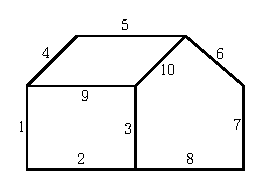
\includegraphics{images/chap5/q19.eps}
\end{figure}

\item 
~

\begin{figure}[H]
\centering
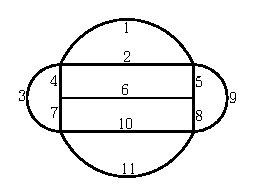
\includegraphics{images/chap5/q20.eps}
\end{figure}

ಈ ಚಿತ್ರ ಗಮನಿಸಿ. ಎಲ್ಲ ರೇಖೆಗಳ ಮೇಲೂ ಪೆನ್ಸಿಲ್ ಎತ್ತದೆ ಚಲಿಸಬೇಕು. ಹಿಮ್ಮುಖ ಚಲನೆ, ಒಂದು ರೇಖೆಯ ಮೇಲೆ 2 ಬಾರಿ ಚಲಿಸುವಂತಿಲ್ಲ. 

\item ಯೂಥಾತ್ಪಂಚಾಂಶಕಸ್ತ್ರ್ಯೂ ನೋವರ್ಗಿತೋ ಗಹ್ವರಂಗತಃ 

ದೃಷ್ಟಃ ಶಾಖಾ ಮೃಗಃ ಶಾಖಾ ಮಾರೂಢೋ ವದತೇ ಕತಿ ।।

\smallskip
\hfill (ಭಾಸ್ಕರಾಚಾರ್ಯರ `ಲೀಲಾವತೀ'ಯಿಂದ)

{\bf ಅರ್ಥ:} ಒಂದು ಗುಂಪಿನಲ್ಲಿದ್ದ ಕೋತಿಗಳಲ್ಲಿ $\frac{1}{5}$ ಭಾಗಕ್ಕೆ 3 ಕಡಿಮೆಯಾದ ಸಂಖ್ಯೆಯ ವರ್ಗದಷ್ಟು ಒಂದು ಗುಹೆಯೊಳಕ್ಕೆ ಹೋದುವು. ಉಳಿದ ಒಂದು ಕೋತಿ ಮರವನ್ನೇರುತ್ತಾ ಇದ್ದಿತು. ಒಟ್ಟು ಕೋತಿಗಳೆಷ್ಟು? 

\item ಯದಿ ಸಮಭುವಿ ವೇಣು ರ್ದ್ವಿ ತ್ರಿಪಾಣಿ ಪ್ರಮಾಣೋ 

ಗಣಕ ಪವನಾ ವೇಗಾದೇಕ ದೇಶೇ ಸಭಗ್ನಃ ।

ಭುವಿ ನೃಪಮಿತ ಹಸ್ತೇಷ್ವಂಗ ಲಗ್ನಂ ತದಗ್ರಂ 

ಕಥಯ ಕತಿಷು ಮೂಲಾದೇಷ ಭಗ್ನ ಕರೇಷು ।।

\smallskip
\hfill (ಭಾಸ್ಕರಾಚಾರ್ಯರ ``ಲೀಲಾವತೀ"ಯಿಂದ)

{\bf ಅರ್ಥ:} ನೆಟ್ಟಗೆ ನಿಂತಿರುವ ಒಂದು ಬೊಂಬು 32 ಮೊಳ ಉದ್ದವಿದೆ. ಗಾಳಿಯ ಹೊಡೆತದಿಂದ ಅದು ಒಂದು ಕಡೆ ಮುರಿದು, ಅದರ ತುದಿಯು ಬುಡದಿಂದ 16 ಮೊಳ ದೂರದಲ್ಲಿ ಭೂಮಿಗೆ ತಗಲುತ್ತದೆ. ಎಲೈಗಣಕನೇ ಬುಡದಿಂದ ಅದು ಎಷ್ಟು ಎತ್ತರದಲ್ಲಿ ಮುರಿದಿದೆ? 

\item ಒಂದು ಜಾನಪದ ಸಮಸ್ಯೆ 

ಒಂಭತ್ತು ರಂಭೆಯರಿಗವನೊಬ್ಬ ಗಂಡ 

ಎಂಭತ್ತೊಂದು ಎಮ್ಮೆಗಳ ತಾ ಕೊಂಡು ತಂದ 

ಕುಂಭ ಕುಂಭಕೆ ಹೆಚ್ಚು ಹಾಲು ಕರಕೊಂಡ 

ರಂಭೆಯರಿಗೆ ಇದ ಸಮ ಮಾಡಿಕೊಳ್ಳಿರೆಂದ 

{\bf ಆಶಯ :} ಒಬ್ಬ ಕವಾಡಿಗ (ಹಾಲು ಮಾರುವವನು). ಅವನಿಗೆ 9 ಹೆಂಡತಿಯರು. 81 ಎಮ್ಮೆಗಳನ್ನು ಕೊಂಡು ತರುತ್ತಾನೆ. 1ನೆ ಎಮ್ಮೆ 1 ಅಳತೆ, 2ನೆ ಎಮ್ಮೆ  2 ಅಳತೆ . . . .  81ನೆ ಎಮ್ಮೆ 81 ಅಳತೆ ಹಾಲು ಕೊಡುತ್ತದೆ. ಹೆಂಡತಿಯರಿಗೆ ರಾಸೂ ಸಮ, ಹಾಲೂ ಸಮ ಆಗುವಂತೆ ಹಂಚಿ. 

\item ಅಂಕಿ ಆಟ. ಯಾವುದಾದರೂ ಸಂಖ್ಯೆ, ಎಷ್ಟಾದರೂ ಅಂಕಿ ಹೇಳಿ. ನಾನು ಹೇಳುವ ಅಂಕಿಯನ್ನು ಮೊದಲಲ್ಲಿ, ಮಧ್ಯದಲ್ಲಿ ಕೊನೆಯಲ್ಲಿ ಎಲ್ಲಿ ಬೇಕಾದರೂ ಬರೆಯಿರಿ. ಬರುವ ಸಂಖ್ಯೆ 3 ರಿಂದ ನಿಶ್ಶೇಷವಾಗಿ ಭಾಗವಾಗುತ್ತದೆ.

\item ನಾಲ್ಕಂಕಿಯ ಒಂದು ಸಂಖ್ಯೆ ಬರೆಯಿರಿ. ತಿರುವು ಮುರುವು ಮಾಡಿ ದೊಡ್ಡ ಸಂಖ್ಯೆಯಲ್ಲಿ ಚಿಕ್ಕದನ್ನು ಕಳೆಯಿರಿ. ಉತ್ತರದಲ್ಲಿ ಯಾವುದಾದರೂ ಒಂದು ಅಂಕಿ ಹೊಡೆದು ಹಾಕಿ. ಉಳಿದ ಅಂಕಿಗಳ ಮೊತ್ತ ಹೇಳಿ. ಹೊಡೆದು ಹಾಕಿದ ಅಂಕಿ ಹೇಳುತ್ತೇನೆ.

\item ಈ ಸಮಯದ ವಿಶಿಷ್ಟತೆ ಏನು?

ಆರನೇ ಮೇ 1978 ಮಧ್ಯಾಹ್ನ 12 ಗಂಟೆ 34 ನಿಮಿಷ 

\item 2 ಅಡಿ ವ್ಯಾಸದ ಅರ್ಧ ಗೋಲಾಕೃತಿಯ ಬೋಗುಣಿಯನ್ನು ಮಳೆಯಲ್ಲಿ ಇರಿಸಿದೆ. ಮಳೆನಿಂತ ನಂತರ ಬೋಗು‌ಣಿಯಲ್ಲಿನ ನೀರಿನ ಆಳ 6". ಈ ನೀರನ್ನು 2 ಅಡಿ ವ್ಯಾಸದ ಸ್ತಂಭಾಕೃತಿ ಪಾತ್ರೆಗೆ ಹಾಕಿದರೆ, ನೀರು ಎಷ್ಟು ಎತ್ತರ ನಿಲ್ಲುತ್ತದೆ? 

\item ಒಬ್ಬ ಸೌದೆ ವ್ಯಾಪಾರಿಯು 40KG ತೂಕದ ಕಲ್ಲನ್ನು ಬಳಸಿ ಸೌದೆ ತೂಗುತ್ತಿದ್ದ. 20KG ಕೇಳಿದವರಿಗೆ 40KG ತೂಗಿ, ಅದನ್ನು 2 ಸಮಭಾಗವಾಗಿ ತೂಗಿಸಿ ಕೊಡುತ್ತಿದ್ದ. ಹೀಗೆಯೇ 10, 5 ಇತ್ಯಾದಿ. ಒಮ್ಮೆ ಕಲ್ಲು ಕೆಳಗೆ ಬಿದ್ದು 4 ಭಾಗವಾಯಿತು. ಅವುಗಳನ್ನು ತ್ರಾಸಿನ ತಟ್ಟೆಗಳಲ್ಲಿಟ್ಟು ಮೊತ್ತ-ವ್ಯತ್ಯಾಸದಿಂದ 1 ರಿಂದ 40KG ವರೆಗೆ ತೂಗಬಹುದೆಂದು ಕಂಡುಕೊಂಡ. ಪ್ರತಿ ಚೂರಿನ ತೂಕವೆಷ್ಟು? 

\item ಒಂದು ಕೊಳದಲ್ಲಿ ವಿಚಿತ್ರ ಹೂ ಇದೆ. ಪ್ರತಿದಿನ ಅದು ತನ್ನ ವಿಸ್ತೀರ್ಣವನ್ನು ದ್ವಿಗುಣಗೊಳಿಸುತ್ತದೆ. 20 ದಿನಗಳಲ್ಲಿ ಅದು ಕೊಳವನ್ನು ಪೂರ್ಣ ಆವರಿಸುತ್ತದೆ. ಕೊಳದಲ್ಲಿ ಇಂತಹ 2 ಹೂಗಳಿದ್ದರೆ ಎಷ್ಟು ದಿನಗಳಲ್ಲಿ, ಕೊಳವನ್ನು ಪೂರ್ಣ ಆವರಿಸುತ್ತದೆ?

\item 100 ಮೀಟರ್ ಉದ್ದದ ಟೇಪಿನ ಒಂದು ಸುರುಳಿ ಇದೆ. ಅದರಿಂದ 1 ಮೀಟರ್ ಉದ್ದದ ಟೇಪು ಕತ್ತರಿಸಲು 1 ಸೆಕೆಂಡ್ ಬೇಕು. 1 ಮೀಟರ್ ಉದ್ದದ 100 ಟೇಪು ಕತ್ತರಿಸಲು ಎಷ್ಟು ಸಮಯಬೇಕು? 
\end{enumerate}

\eject

\begin{center}
\rule{5cm}{1pt}\\[3pt]
{\Large\bfseries ಉತ್ತರಗಳು}\\[-0.1cm]
\rule{5cm}{1pt}
\end{center}

\begin{enumerate}
\itemsep=5pt

\item $44+44+4+4+4 = 100$

\item $16+16+17+17+17+17 = 100$

\item $3+3\times 3 - 3 \div 3 - 3$ ಬೋದ್‌ಮಾಸ್ ನಿಯಮದಂತೆ $\div, \times, +, -$ ಕ್ರಮವಾಗಿ

\begin{tabular}[t]{ll}
$3+3\times 3 - 1 - 3$ & $(3 \div 3 = 1)$\\
$3+9 - 1 - 3$ & $(3 \times 3 = 9)$\\
$12 - 4 = 8$ & 
\end{tabular}

\item $44 + \dfrac{44}{4} = 44 + 11 = 55$

\item ವ್ಯತ್ಯಾಸದಲ್ಲಿ 36 ಕಳೆಯಿರಿ, 12 ರಿಂದ ಭಾಗಿಸಿ. ಅವರ ಸಂಖ್ಯೆ ಲಭ್ಯ. 

ಉದಾ: 53 ಇರಲಿ 

$53 + 6 =  59 \qquad 53^{2} = 2809 \quad 59^{2} = 3481$
\begin{align*}
3481 - 2809 & = 672\\
672 - 36 & = 36\\
\dfrac{636}{12} & = 53
\end{align*}

\item ಅವರು ಹೇಳುವ ಉತ್ತರದಲ್ಲಿ, 50 ಕಳೆದರೆ ಮೊದಲ ಸಂಖ್ಯೆ ಲಭ್ಯ. 

ಉದಾ: 435 ಇರಲಿ 
{\fontsize{11pt}{13pt}\selectfont
\begin{tabbing}
$(4\times 2) + 1 = 9$ \= ; \= $\quad 9\times 5 ~;~  45+3 = 48$\\
$48\times 10 = 480$ \> ; \> $\quad 480 + 5 = 485$\\
$\quad485 - 50$ \> = \> $\quad 435$
\end{tabbing}}\relax

\item
\begin{tabular}[t]{llll}
(a)& II $+$ I = III & (b)& V $+$ IV = IX\\
(c)& V $-$ III = II &(d)& IV $-$ III = 1\\
(e)& X $+$ I = XI & & \\
& IX $+$ I = X & &
\end{tabular}

\item 
~

\begin{tabular}[t]{ll}
\includegraphics{images/chap5/ans8a.eps} & {$0$ ಗುರುತಿಸಿದನ್ನು ತೆಗೆದು ಹಾಕಿದೆ.}\\
\includegraphics{images/chap5/ans8.eps} & \raisebox{.7cm}{$\checkmark$ ಗುರುತಿಸಿದನ್ನು ಅಡ್ಡಲಾಗಿಸಿದೆ.}
\end{tabular}


\smallskip
\item
~

\begin{minipage}[c]{3cm}
\begin{figure}[H]
\centering
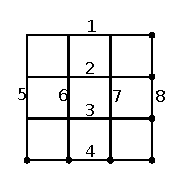
\includegraphics{images/chap5/ans9a.eps}
\end{figure}
\end{minipage}
\begin{minipage}[c]{3cm}
\begin{figure}[H]
\centering
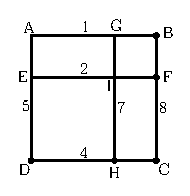
\includegraphics{images/chap5/ans9.eps}
\end{figure}
\end{minipage}
\begin{minipage}[c]{3cm}
3, 6 ನ್ನು ತೆಗೆದಿದೆ
\begin{align*}
& \left.
\begin{aligned}
\text{EDHI} \\
\text{GIFB} \\
\text{ABCD} 
\end{aligned}
\right\}
~~  \text{ಚೌಕಗಳು}\\
& \left.
\begin{aligned}
\text{AGIE} \\
\text{IFCH}
\end{aligned}
\right\}
~~  \text{ಆಯತಗಳು}
\end{align*}
\end{minipage}

\item
~

\begin{figure}[H]
\centering
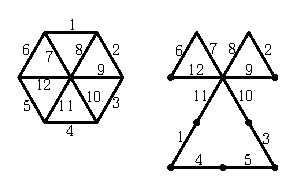
\includegraphics[scale=1.4]{images/chap5/ans10.eps}
\end{figure}

\item
~

\begin{minipage}[c]{4cm}
\begin{figure}[H]
\centering
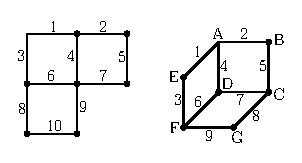
\includegraphics[scale=1.2]{images/chap5/ans11.eps}
\end{figure}
\end{minipage}
\qquad\qquad
\begin{minipage}[c]{4cm}
\begin{align*}
& \text{ABCD  ಚೌಕ }\\
& \left.
\begin{aligned}
\text{AEFD} \\
\text{FDCE}
\end{aligned}
\right\}
~~  \text{ವಜ್ರಾಕೃತಿ}\\
& 10 \text{ ನ್ನು ತೆಗೆದಿದೆ }
\end{align*}
\end{minipage}

\eject

\item
~
\vskip -0.8cm
\begin{figure}[H]
\centering
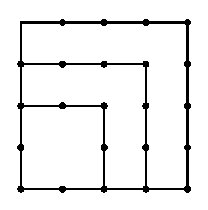
\includegraphics{images/chap5/ans12.eps}
\end{figure}

\item
\begin{tabular}[t]{l@{\;}l@{\;}l}
$9999 \times 5$ & = & $4~999~5$\\
$9999 \times 6$ & = & $5~999~4$\\
$9999 \times 7$ & = & $6~999~3$\\
$9999 \times 8$ & = & $7~999~2$\\
$9999 \times 9$ & = & $8~999~1$
\end{tabular}

\item
{\fontsize{5}{7}\selectfont{
\begin{align*}
1234321 & = \dfrac{4444\times 4444}{1+2+3+4+3+2+1}\\[0.2cm]
123454321 & = \dfrac{55555\times 55555}{1+2+3+4+5+4+3+2+1}\\[0.2cm]
12345654321 & = \dfrac{666666+666666}{1+2+3+4+5+6+5+4+3+2+1}\\[0.2cm]
1234567654321 & = \dfrac{7777777+7777777}{1+2+3+4+5+6+7+6+5+4+3+2+1}\\[0.2cm]
123456787654321 & = \dfrac{88888888+88888888}{1+2+3+4+5+6+7+8+7+6+5+4+3+2+1}\\[0.2cm]
12345678987654321 & = \dfrac{999999999+999999999}{1+2+3+4+5+6+7+8+9+8+7+6+5+4+3+2+1}
\end{align*}}}

\item
\begin{tabular}[t]{l@{\;}c@{\;}l}
$3333\times 3335$ & = & $1111~5555$\\
$33333\times 33335$ & = & $11111~55555$\\
$333333\times 333335$ & = & $111111~555555$
\end{tabular}

\item
\begin{tabular}[t]{r@{\;}c@{\;}r}
$200001^{2}$ & = & $40000~400001$\\
$2000001^{2}$ & = & $400000~4000001$\\
$20000001^{2}$ & = & $4000000~40000001$
\end{tabular}

\item $2^{5} \cdot 9^{2}\qquad \cdot$ ಎಂದರೆ ಗುಣಿಸು

$2592$ ಘಾತವನ್ನು ಪಕ್ಕದಲ್ಲಿ ಬರೆದಿದೆ. 
\begin{align*}
2^{5} & = 2\times 2\times 2\times 2 = 32\\
9^{2} & = 81\\
& \qquad 32\times 81 = 2592
\end{align*}

\item
~

\begin{minipage}[c]{4cm}
2 ತ್ರಿಭುಜಗಳ ಬಾಹುಗಳು 6 

ಇವು ಸಾಲುಗಳು 

ಪ್ರತಿ ಸಾಲಿನಲ್ಲೂ 4 ಸಸಿಗಳಿವೆ 

(1 ರಿಂದ 12 ಸಸಿಗಳು)
\end{minipage}
\begin{minipage}[c]{5cm}
\begin{figure}[H]
\centering
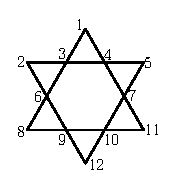
\includegraphics{images/chap5/ans18.eps}
\end{figure}
\end{minipage}

\item
~

\begin{minipage}[c]{5cm}
\begin{figure}[H]
\centering
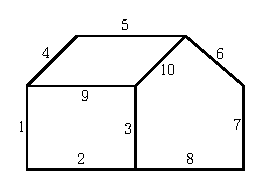
\includegraphics{images/chap5/q19.eps}

\text{ಕೊಟ್ಟಿದ್ದು}
\end{figure}
\end{minipage}
\begin{minipage}[c]{4cm}
\begin{figure}[H]
\centering
\text{9, 10 ಬದಲಿಸಿದೆ.}
\includegraphics{images/chap5/ans19.eps}
\text{ರಚಿಸಿದ್ದು}
\end{figure}
\end{minipage}

\item
~

\begin{figure}[H]
\centering
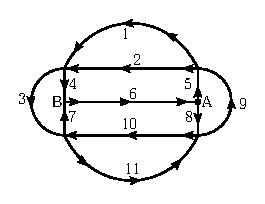
\includegraphics[scale=1.1]{images/chap5/ans20.eps}

\text{A ಯಿಂದ ಪ್ರಾರಂಭಿಸಿ 5, 2, 4, 6, 8, 10, 11, 9, 1, 3, 7, B}
\end{figure}


\item
\begin{tabular}[t]{rl}
& ಯೂಥಾತ್ಪಂಚಾಂಶಕ ಸ್ತ್ರೋನೋ ವರ್ಗಿತೋಗಹ್ವರಂ ಗತಃ ।\\
& ದೃಷ್ಟಃ ಶಾಖಾಮೃಗಃ ಶಾಖಾಮಾರೂ ಢೋ ವದತೇ ಕತಿಃ ।। \\[0.1cm]
& \qquad \hfill{(ಭಾಸ್ಕರಾಚಾರ್ಯರ `ಲೀಲಾವತಿ'ಯಿಂದ)}
\end{tabular}

ಕೋತಿಗಳ ಸಂಖ್ಯೆ $x$ ಇರಲಿ
\begin{align*}
\left(\dfrac{x}{5} - 3 \right)^{2} + 1 & = x\\
\dfrac{x^{2}}{25} - \dfrac{6x}{5} + 9 + 1 & = x\\
x^{2} - 30x + 250 & = 25x\\
x^{2} - 55x + 250 & = 0\\
(x - 5)(x - 50) & = 0\\
x = 5,\quad x = 50 &
\end{align*}

5 ಸಾಧ್ಯವಿಲ್ಲ $\quad\therefore$ ಕೋತಿಗಳ ಸಂಖ್ಯೆ  50

\item
~

\begin{minipage}[c]{4cm}
AB ಬೊಂಬು ಇರಲಿ 

AB = 32 ಮೊಳ 

AD = 16 ಮೊಳ 

AC = x ಆದರೆ

BC = CD = 32 $-$ x
\end{minipage}
\begin{minipage}[c]{5cm}
\begin{figure}[H]
\centering
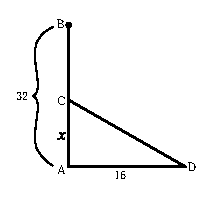
\includegraphics[scale=1.2]{images/chap5/ans22.eps}
\end{figure}
\end{minipage}

\begin{align*}
x^{2} + 16^{2} & = (32 - x)^{2}\\
x^{2} + 256 & = 1024 - 64x + x^{2}\\
64x & = 1024 - 256\\
x & = \dfrac{768}{64} = 12~\text{ ಮೊಳ}
\end{align*}

\item ಇದಕ್ಕೆ ಪರಿಹಾರ 9 ಮನೆಯ ಮಾಯಾ ಚೌಕ.
\begin{figure}[H]
\centering
\includegraphics[scale=1.2]{images/chap5/ans23.eps}
\end{figure}

ಒಟ್ಟು ಎಮ್ಮೆಗಳು 81  \qquad $\therefore$ ಒಬ್ಬರಿಗೆ 9 ಎಮ್ಮೆ 

\smallskip
ಒಟ್ಟು ಹಾಲು $1+2+3\cdots + 81 = \dfrac{81 \times 81}{2} = 3321$

\smallskip
9 ಜನರಿಗೆ ಹಂಚಿದಾಗ $\dfrac{3321}{9} = 369$~ ಅಳತೆ 

ಯಾವುದೇ ಅಡ್ಡ ಸಾಲು, ಕಂಭ ಸಾಲು ಕೂಡಿದರೆ 369 ಬರುತ್ತದೆ. ಆ ಸಂಖ್ಯೆಗಳ ಎಮ್ಮೆ ಹಂಚಿಕೆಯಾಗಬೇಕು. 

\item ಅವರ ಸಂಖ್ಯೆಯ ಅಂಕಿಗಳ ಮೊತ್ತ (ಒಂದಂಕಿ) ಲೆಕ್ಕಿಸಿ. ಅದರ ಮುಂದಿನ 9ರ ಅಪವರ್ತ್ಯದಲ್ಲಿ ಕಳೆಯಿರಿ. ಉತ್ತರದ ಅಂಕಿಯನ್ನು ಸೇರಿಸಿಕೊಳ್ಳಲು ಹೇಳಿ. 

\smallskip
ಉದಾ: (1) $76342\quad 7+6+3+4+2 = 22 ~~;~~ 2+2 = 4$

\quad ಮುಂದಿನ ಅಪವರ್ತ್ಯ $9$;~ $9 - 4 = 5~$ ಇದನ್ನು ಎಲ್ಲಿ ಬೇಕಾದರೂ ಸೇರಿಸಲಿ. ಸಂಖ್ಯೆ 3 ರಿಂದ ನಿಶ್ಶೇಶ ಭಾಗವಾಗುತ್ತದೆ.   

\smallskip
ಉದಾ: (2) $80148763 ~~;~~ 8+0+1+4+8+7+6+3 = 37$

$3 + 7 = 10 ~~;~~ 1 + 0 = 1$

\quad ಮುಂದಿನ ಅಪವರ್ತ್ಯ $9$.\quad $9 - 1 = 8$

$\therefore\quad 8$ ನ್ನು ಸೇರಿಸಲಿ 

\item ಉದಾ: (1) 5493 ಅದರ ಸಂಖ್ಯೆ ಇರಲಿ. ತಿರುವು ಮುರುವು 3945
\begin{equation*}
\begin{tabular}[t]{l}
$5493$\\
$3945$\\
\hline
$1548$
\end{tabular}
\quad 1\cancel{5}48\quad 5 \text{ ನ್ನು ಹೊಡೆದು ಹಾಕುತ್ತಾರೆಂದು ಇಟ್ಟುಕೊಳ್ಳೋಣ.}
\end{equation*}

ಉಳಿದ ಅಂಕಿಗಳ ಮೊತ್ತ 13

9 ರ ಮುಂದಿನ ಅಪವರ್ತ್ಯ $18\qquad \therefore\quad 18 - 13 = 5$ ಹೊಡೆದಿರುವುದು

\smallskip
ಉದಾ: (2) 
\begin{tabular}[t]{llr}
$6187$ & $7861$ & $1 + 6 + 9 = 16$\\
& $6187$ & $18 - 16 = 2$\\
\cline{2-2}
& $16\cancel{2}9$ & 
\end{tabular}

ಅಥವಾ ಒಂದಂಕಿ ಮೊತ್ತ ಬರಿಸಿ 

\smallskip
ಉದಾ: (1) ರಲ್ಲಿ $1 + 3 = 4\quad 9$ರಲ್ಲಿ ಕಳೆಯಿರಿ $9 - 4 = 5$

ಉದಾ: (2) ರಲ್ಲಿ $1 + 6 + 9 = 16 = 18 - 6 = 2$

\smallskip
\item $\dfrac{12}{\text{ಗಂ}}\quad \dfrac{34}{\text{ನಿ}}\quad \dfrac{5}{\text{ತಿಂ}}\quad \dfrac{6}{\text{ದಿನ}}\quad \dfrac{78}{\text{ಇಸವಿ}}$

\smallskip
\item 
~

\begin{minipage}[c]{4cm}
OM = r = 12"

 PN = h = 6"
\end{minipage}
\begin{minipage}[c]{5cm}
\begin{figure}[H]
\centering
\includegraphics[scale=1.2]{images/chap5/ans27.eps}
\end{figure}
\end{minipage}

ಗೋಲದ ಖಂಡಭಾಗದ ಗಾತ್ರ $V = \dfrac{1}{3} \Pi~ h^{2}~ (3r - h)$ \{ಸೂತ್ರ\}

r = 12"\qquad h = 6"
\begin{align*}
\therefore\quad V & = \dfrac{1}{3} \times \Pi \times 6^{2} (36 - 6)\\[0.2cm]
& = \dfrac{1}{\cancel{3}} \times \Pi \times \cancel{36}^{12} \times 30 = 360 \Pi
\end{align*}

\eject

ಸ್ತಂಭಾಕೃ ತಿಯ ಗಾತ್ರ = $\Pi~ r^{2}h$

r = 12",\qquad h = ?
\begin{align*}
\Pi(12)^{2} (h) & = 360~ \Pi\\
144~h & = 360\\
h & = \dfrac{360}{144} = \dfrac{30}{12} = \dfrac{5}{2} = 2\dfrac{1}{2}\text{"}
\end{align*}

\item ಚೂರುಗಳು $1, 3, 9, 27$ ಕೆಜಿ. $\left(3^{0}, 3^{1}, 3^{2}, 3^{3}\right)$

$2$ ಬೇಕಾದರೆ $1 - 3$

$20$ ಬೇಕಾದರೆ $27, 3 - 9, 1$

$5$ ಬೇಕಾದರೆ $9 - 3, 1$~ ಇತ್ಯಾದಿ 

\item 19 ದಿನ \{1 ಹೂ ಇದ್ದರೆ 20 ದಿನಗಳಲ್ಲಿ ಪೂರ್ಣ ಆವರಿಸುತ್ತದೆ. ಅದು 19 ದಿನಗಳಲ್ಲಿ $\frac{1}{2}$ ಕೊಳ ಆವರಿಸುತ್ತದೆ. ಇನ್ನೊಂದು ಹೂ ಇದ್ದರೆ ಅದು 19 ದಿನಗಳಲ್ಲಿ $\frac{1}{2}$ ಕೊಳ ಆವರಿಸುತ್ತದೆ.\}

\item 99 ಸೆಕೆಂಡ್ 99 ಸಲ ಕತ್ತರಿಸಿದರೆ 100 ಚೂರುಗಳಾಗುತ್ತದೆ.
\end{enumerate}
